\documentclass[a4paper, oneside, 10pt]{book}
\usepackage{graphicx}
\usepackage{float}
\usepackage{adjustbox}
\usepackage{listings}
\usepackage{fullpage}
\usepackage{booktabs}
\usepackage{subfig}
\usepackage{enumerate}
\usepackage{pgfplots}
\pgfplotsset{compat=1.8}
\usepackage{tabularx}
\usepackage{multirow}
\usepackage[T1]{fontenc}
\usepackage{inputenc}
\usepackage{hyperref}
\usepackage[italian]{babel}
\usepackage{longtable} 
\usepackage{mathtools}
\usepackage{amssymb,amsmath,amsthm}

\definecolor{codegreen}{rgb}{0,0.6,0}
\definecolor{codegray}{rgb}{0.5,0.5,0.5}
\definecolor{codepurple}{rgb}{0.58,0,0.82}
\definecolor{backcolour}{rgb}{0.95,0.95,0.92}

\lstdefinestyle{mystyle}{
    backgroundcolor=\color{backcolour},   
    commentstyle=\color{codegreen},
    keywordstyle=\color{magenta},
    numberstyle=\tiny\color{codegray},
    stringstyle=\color{codepurple},
    basicstyle=\ttfamily\footnotesize,
    breakatwhitespace=false,         
    breaklines=true,                 
    captionpos=b,                    
    keepspaces=true,                 
    numbers=left,                    
    numbersep=5pt,                  
    showspaces=false, 
    showlines=false,               
    showstringspaces=false,
    showtabs=false,                  
    tabsize=2,
    morekeywords={*, REFERENCES, ENABLED, DISABLED, IS, BEFORE, AFTER, INCREMENT, START, WITH, SEQUENCE, FOR, EACH, ROW, INSTEAD OF, FOR EACH STATEMENT}
}
\lstset{
style= mystyle
}
\def\ojoin{\setbox0=\hbox{$\bowtie$}%
  \rule[-.02ex]{.25em}{.4pt}\llap{\rule[\ht0]{.25em}{.4pt}}}
\def\leftouterjoin{\mathbin{\ojoin\mkern-5.8mu\bowtie}}
\def\rightouterjoin{\mathbin{\bowtie\mkern-5.8mu\ojoin}}
\def\fullouterjoin{\mathbin{\ojoin\mkern-5.8mu\bowtie\mkern-5.8mu\ojoin}}
\begin{document}

\begin{titlepage}
\begin{center}


\includegraphics[scale=0.6]{Immagini/logo_dieti.png}
\vspace*{1cm}

{\Huge{\textbf{Progettazione e sviluppo di una base di dati relazionale per la gestione di conferenze scientifiche}}}

\vspace{1cm}

{\Large Progetto d'esame per il corso di Basi di Dati}


\vfill

{\Large Caporaso Antonio} \qquad \Large{Di Fusco Giorgio}\\
\texttt{N86003458} \qquad \texttt{N86004389}\\

\vspace{1cm}

Docente: Sangiovanni Mara\\

\vspace{1cm}


\includegraphics[scale=0.6]{Immagini/LogoUnina.png}


\begin{small}
Corso di Laurea Triennale in Informatica \textsc{A.A 2022/2023}\\
Dipartimento di Ingegneria Elettrica e delle tecnologie dell'Informazione\\
Università degli Studi di Napoli Federico II
\end{small}
\end{center}
\end{titlepage}
\newpage
\textit{Questa pagina è stata lasciata intenzionalmente vuota.}
\newpage
\tableofcontents
\listoffigures
\listoftables
\chapter{Traccia}\label{sez:traccia}
Si sviluppi un sistema informativo, composto da una base di dati relazionale e da un applicativo Java dotato
di GUI (Swing o JavaFX), per la gestione di \textbf{conferenze scientifiche}. 
\bigskip

Ogni conferenza ha una data di inizio e di fine, una collocazione (sede, indirizzo), uno o più enti che la organizzano, degli sponsor (che coprono in parte le spese), una descrizione, ed un gruppo di organizzatori, che può essere distinto in comitato scientifico e comitato locale (che si occupa cioè della logistica). Di ognuno degli organizzatori, così come di tutti i partecipanti, si riportano titolo, nome, cognome, email ed istituzione di afferenza. 
\bigskip

Ogni conferenza può avere una o più sessioni, anche in parallelo fra loro. Ogni sessione ha una locazione all'interno della sede. Per ogni
sessione c'è un programma, che prevede la presenza di un coordinatore (chair) che gestisce la sessione, ed eventualmente di un keynote speaker (un partecipante di particolare rilievo invitato dagli organizzatori). Ogni sessione avrà quindi una successione di interventi ad orari predefiniti e di specifici partecipanti. Per ogni intervento si conserva un abstract (un breve testo in cui viene spiegato il contenuto del lavoro presentato).
\bigskip

Si deve poter considerare la presenza di spazi di intervallo (coffee breaks, pranzo) ma anche la presenza di eventi sociali (cene, gite, etc).
\section{Output attesi dal committente}
\begin{enumerate}
\item Documento di Design della base di dati:
\begin{enumerate}
\item Class Diagram della base di dati.
\item Dizionario delle Classi, delle Associazioni e dei Vincoli.
\item Schema Logico con descrizione di Trigger e Procedure individuate.
\end{enumerate}
\item File SQL contenenti:
\begin{enumerate}
\item Creazione della struttura della base di dati.
\item Popolamento del DB.
\item (Facoltativo, ma apprezzato) README contenente i commenti all’SQL.
\end{enumerate}
\end{enumerate}
\chapter{Progettazione concettuale}
\section{Analisi dei dati}
Le entità che possono essere individuate nel problema sono elencate all'interno della Tabella \ref{tab:entities}.
\begin{table}[h!]
\begin{tabularx}{\textwidth}{|l|X|}
\hline
\textbf{Entità} & \textbf{Descrizione} \\
\hline
\textbf{Conferenza} & Per le conferenze delle quali si vuole poter gestire le informazioni. Di ogni conferenza si conservano il \textit{nome}, la \textit{data di inizio} e di \textit{fine} e una \textit{descrizione}. \\ \hline
\textbf{Ente} & Per gli enti che organizzano le conferenze scientifiche. Di ogni ente si conserva solo il \textit{nome}. \\ \hline
\textbf{Sponsor} & Per gli sponsor che coprono le spese della conferenza. Di ogni sponsor si conserve solo il \textit{nome}.\\ \hline
\textbf{Comitato} & Per i gruppi di organizzatori che si occupano della gestione della conferenza scientifica. Si distinguono in comitati \textit{scientifici} e \textit{locali}. \\ \hline
\textbf{Organizzatore} & Per i membri dei comitati scientifici e locali. Di ogni organizzatore si riportano \textit{titolo, nome, cognome, email} ed \textit{istituzione di afferenza}. \\ \hline
\textbf{Sede} & Per descrivere il luogo dove si tengono le varie conferenze. Di ogni sede si conservano: \textit{nome, indirizzo, città} e il \textit{codice di indirizzamento postale}. \\ \hline
\textbf{Sala} & Per tenere traccia dell'ubicazione delle varie sessioni. Di ogni sala si conserva il \textit{nome della sala} e la sua \textit{capacità}. \\ \hline
\textbf{Sessione} & Per rappresentare le sessioni di una conferenza. Per ogni sessione si riporta il \textit{titolo} e le date di \textit{inizio} e di \textit{fine}. \\ \hline
\textbf{Programma} & Per il programma di ciascuna sessione. Ogni programma contiene la specifica del \textit{coordinatore} della sessione ed eventualmente la presenza di un \textit{keynote speaker}, ovvero un partecipante di rilievo. \\ \hline
\textbf{Intervento} & Per i vari interventi di una sessione. Per ogni intervento si conserva un \textit{abstract}, il partecipante (\textit{speaker}) che effettua l'intervento e l'\textit{orario} dello stesso. \\ \hline
\textbf{Partecipante} & Per i partecipanti delle varie sessioni. Ogni partecipante ha gli stessi attributi degli organizzatori. \\ \hline
\textbf{Intervallo} & Per descrivere i vari intervalli presenti all'interno di una sessione. Questi possono essere di tue tipologie: coffee break oppure dei pranzi. Per ogni intervallo si riporta l'\textit{orario}. \\ \hline
\textbf{Evento sociale} & Per i vari eventi sociali previsti all'interno di una sessione. Questi possono essere di varia natura. Come per gli intervalli se ne riporta l'\textit{orario}. \\ \hline
\textbf{Utente} & Per l'utente di un applicativo che interagisce con la base di dati. Di ogni utente si conservano gli stessi dati di un organizzatore. In aggiunta è presente un attributo per la \textit{password}. \\
\hline
\end{tabularx}
\caption{}\label{tab:entities}
\end{table}
\newpage
\section{Schema concettuale}
\begin{figure}[h!]
\centering
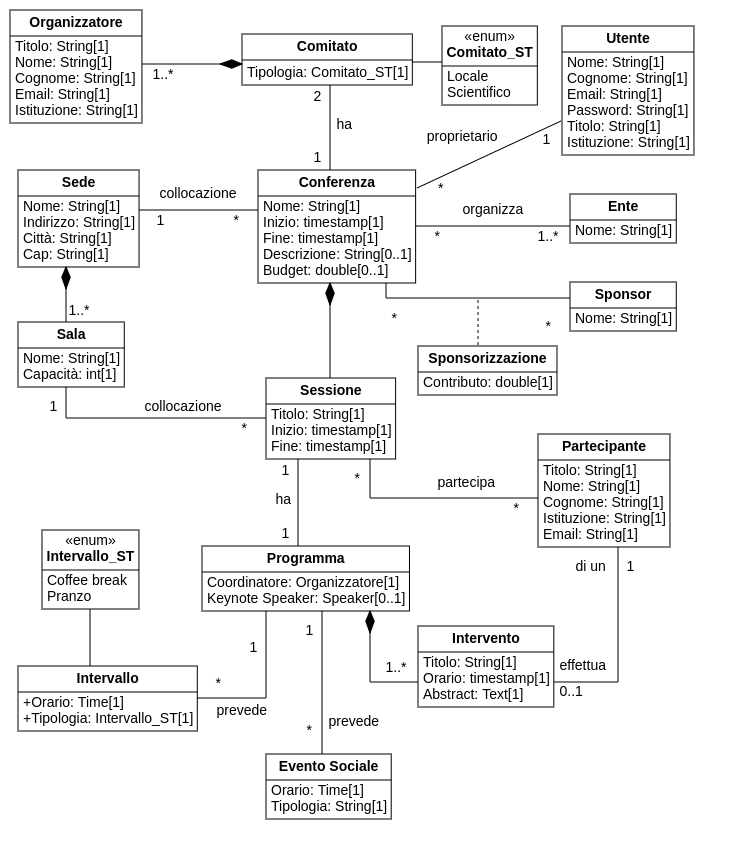
\includegraphics[scale=0.6]{Immagini/Schema_Concettuale.png}
\caption{Schema concettuale del problema}\label{uml:schema_concettuale}
\end{figure}
Nella Figura \ref{uml:schema_concettuale} è presente lo schema concettuale della base di dati descritta nella sezione \ref{sez:traccia}.
\section{Ristrutturazione dello schema concettuale}


\chapter{Ristrutturazione del Class Diagram}
\chapter{Progettazione logica}
\section{Traduzione delle classi}
\section{Traduzione delle associazioni}
\section{Schema logico}
\chapter{Implementazione fisica}
\section{Definizione delle tabelle}
\section{Popolamento}
\section{Dizionario dei dati}
\begin{longtable}{|p{0.2\textwidth}|p{0.3\textwidth}|p{0.45\textwidth}|}
\hline
\textbf{Classe} & \textbf{Descrizione} & \textbf{Attributi} \\
\hline
\endfirsthead

% Intestazione normale
\multicolumn{3}{l}{\footnotesize\itshape Continua dalla pagina precedente} \\
\hline
\textbf{Classe} & \textbf{Descrizione} & \textbf{Attributi} \\
\hline
\endhead

% Piede normale
\hline
\multicolumn{3}{r}{\footnotesize\itshape Continua nella prossima pagina} \\
\endfoot

% Piede finale
\hline
\endlastfoot

	\textbf{Comitato} & Tabella che descrive i comitati che si occupano della logistica e della pianificazione delle conferenze scientifiche. & \texttt{id\_comitato} (\textit{serial}) (\textit{totale}): Identificatore univoco per un comitato. \\ 
	& & \texttt{tipologia}(\textit{comitato\_st})(\textit{totale}): Specifica il tipo di comitato (scientifico o locale). \\	\hline

	\textbf{Conferenza} & Tabella che descrive le conferenze scientifiche. & \texttt{Id\_Conferenza}(\textit{serial})(\textit{totale}): Chiave primaria per una conferenza. \\
	& & \texttt{Titolo}(\textit{Text}) (\textit{totale}): Specifica il titolo della conferenza scientifica. \\
	& & \texttt{Descrizione}(\textit{Text})(\textit{parziale}): Fornisce una descrizione della conferenza scientifica. \\
	& & \texttt{Inizio}(\textit{Timestamp})(\textit{totale}): Indica l'inizio della conferenza. \\
	& & \texttt{Fine} (\textit{Timestamp})(\textit{totale}) : Indica la fine della conferenza. \\	\hline

	\textbf{Ente} & Tabella delle istituzioni & \texttt{Id\_Ente}(\textit{serial})(\textit{totale}): Identificatore primario di una istituzione. \\
	& & \texttt{Nome}(\textit{Text})(\textit{totale}): Nome dell'istituzione. \\
	& & \texttt{Sigla}(\textit{Varchar(7)})(\textit{totale}) : Sigla dell'istituzione. \\	\hline
	
	\textbf{Evento} & Eventi sociali presenti all'interno di una conferenza.&  \texttt{Id\_Evento}(\textit{Serial})(\textit{Totale}): Identificatore primario per un evento. \\
	& & \texttt{Tipologia}(\texttt{text})(totale): Stringa descrittiva della tipologia dell'evento. \\
	& & \texttt{Inizio}(\textit{Timestamp})(\textit{totale}): Indica l'inizio dell'evento. \\
	& & \texttt{Fine} (\textit{Timestamp})(\textit{totale}) : Indica la fine dell'evento. \\	\hline
	
	\textbf{Indirizzo} & Tabella degli indirizzi per ogni sede & \texttt{Id\_Indirizzo}(\textit{serial})(\textit{totale}): Chiave primaria. \\
	& & \texttt{Via}(\textit{text})(\textit{parziale}): nome della via. \\
	& & \texttt{Civico}(text)(parziale): civico della sede. \\
	& & \texttt{Cap}(char(5))(parziale): codice di avviamento postale \\
	& & \texttt{Città}(text)(parziale): città della sede. \\
	& & \texttt{Provincia}(varchar(2)): provincia della città. \\
	& & \texttt{Stato}(text)(parziale): stato della sede. \\ \hline
	
	\textbf{Intervallo} & Descrittore degli intervalli presenti all'interno di una conferenza scientifica.&  \texttt{Id\_Intervallo}(\textit{Serial})(\textit{Totale}): Identificatore primario per un evento. \\
	& & \texttt{Tipologia}(\textit{Intervallo\_ST})(totale): Specifica il tipo di intervallo (pranzo o coffee break).  \\
	& & \texttt{Inizio}(\textit{Timestamp})(\textit{totale}): Indica l'inizio dell'intervallo. \\
	& & \texttt{Fine} (\textit{Timestamp})(\textit{totale}) : Indica la fine dell'intervallo. \\ \hline
	
	\textbf{Intervento} & Descrittore degli interventi che si tengono all'interno delle sessioni. & \texttt{Id\_Intervento}(\textit{Serial})(\textit{totale}): Identificatore primario di un intervento. \\
	& & \texttt{Titolo}(\textit{Text}) (\textit{totale}): Specifica il titolo dell'intervento. \\
	& & \texttt{Abstract}(\textit{Text})(\textit{parziale}): Fornisce una descrizione dell'intervento. \\
	& & \texttt{Inizio}(\textit{Timestamp})(\textit{totale}): Indica l'inizio dell'intervento. \\
	& & \texttt{Fine} (\textit{Timestamp})(\textit{totale}) : Indica la fine dell'intervento. \\	\hline
	
	\textbf{Organizzatore} & Descrittore dei membri dei comitati. & \texttt{Id\_Organizzatore}(\textit{serial})(\textit{Totale}): Identificatore principale di un organizzatore. \\
	& & \texttt{Nome}(\textit{text})(\textit{totale}): nome dell'organizzatore. \\
	& & \texttt{Cognome}(\textit{text})(\textit{totale}): cognome dell'organizzatore. \\
	& & \texttt{Titolo}(\textit{Titolo\_ST})(\textit{parziale}): Titolo accademico dell'organizzatore \\
	& & \texttt{Email}(\textit{Text})(\textit{Parziale}): Email dell'organizzatore \\	\hline
	
	\textbf{Partecipante} & Descrittore dei partecipanti delle sessioni. & \texttt{Id\_Partecipante}(\textit{serial})(\textit{Totale}): Identificatore principale di un partecipante. \\
	& & \texttt{Nome}(\textit{text})(\textit{totale}): nome dell'organizzatore. \\
	& & \texttt{Cognome}(\textit{text})(\textit{totale}): cognome dell'organizzatore. \\
	& & \texttt{Titolo}(\textit{Titolo\_ST})(\textit{parziale}): Titolo accademico del partecipante. \\
	& & \texttt{Email}(\textit{Text})(\textit{Parziale}): Email del partecipante. \\	\hline
	
	\textbf{Programma} & Tabella dei programmi delle sessioni. & \texttt{Id\_Programma}(\textit{serial})(\textit{totale}): Identificatore principale dei programmi. \\ \hline
	
	\textbf{Sala} & Tabella delle sale di ciascuna sede. & \texttt{Id\_sala}(\textit{serial})(\textit{totale}): identificatore principale di ciascuna sala. \\
	& & \texttt{Nome}(\textit{Text})(\textit{totale}): nome della sala. \\
	& & \texttt{Capienza}(\textit{int})(\textit{totale}): capienza della sala.\\	\hline
	
	\textbf{Sede} & Descrizione delle sedi che ospitano le conferenze & \texttt{Id\_Sede}(\textit{Serial})(\textit{totale}) : Identificatore principale delle sedi. \\
	& & \texttt{Nome}(\textit{Text})(\textit{totale}): nome della sede. \\	\hline
	
	\textbf{Sessione} & Tabella delle sessioni di ciascuna conferenza. & \texttt{Id\_Sessione}(\textit{Serial})(\textit{total}): Identificatore primario di una sessione. \\
	& & \texttt{Titolo}(\textit{Text}) (\textit{totale}): Specifica il titolo della sessione. \\
	& & \texttt{Inizio}(\textit{Timestamp})(\textit{totale}): Indica l'inizio della sessione. \\
	& & \texttt{Fine} (\textit{Timestamp})(\textit{totale}) : Indica la fine della sessione. \\	\hline
	
	\textbf{Speaker} & Descrittore dei vari speaker delle sessioni. & \texttt{Id\_Speaker}(\textit{serial})(\textit{Totale}): Identificatore principale di uno speaker. \\
	& & \texttt{Nome}(\textit{text})(\textit{totale}): nome dello speaker. \\
	& & \texttt{Cognome}(\textit{text})(\textit{totale}): cognome dello speaker. \\
	& & \texttt{Titolo}(\textit{Titolo\_ST})(\textit{parziale}): Titolo accademico dello speaker. \\
	& & \texttt{Email}(\textit{Text})(\textit{Parziale}): Email dello speaker. \\	\hline
	
	\textbf{Sponsor} & Tabella degli sponsor & \texttt{Id\_Sponsor}(\textit{serial})(\textit{totale}): Identificatore primario di uno sponsor. \\
	& & \texttt{Nome}(\textit{Text})(\textit{totale}): Nome dello sponsor. \\ \hline
	
	\textbf{Valuta} & Tabella delle valute & \texttt{Iso} (\textit{Char(3)})(\textit{totale}): codice univoco internazionale delle valute. \\
	& & \texttt{Nome}(\textit{text})(\textit{totale}): nome della valuta. \\
	& & \texttt{Simbolo}(\textit{char(1)})(\textit{totale}): simbolo della valuta.\\
\end{longtable}
\section{Dizionario delle associazioni}
\begin{longtable}{|p{0.35\textwidth}|p{0.3\textwidth}|p{0.3\textwidth}|}
	\hline
	\textbf{Associazione} & \textbf{Descrizione} & \textbf{Classi coinvolte}\\
	\hline
	\endfirsthead
	
	%Intestazione normale
	\multicolumn{3}{l}{\footnotesize\itshape Continua dalla pagina precedente}\\
	\hline
	\textbf{Associazione} & \textbf{Descrizione} & \textbf{Classi coinvolte}\\
	\hline
	\endhead
	%piedenormale
	\hline 
	\multicolumn{3}{r}{{Continua nella pagina successiva}} \\
	\endfoot
	
	\hline
	\endlastfoot
	\textbf{Appartiene\_A} & Rappresenta l'appartenenza di un organizzatore ad una precisa istituzione. & \textbf{Organizzatore [0..*]}: indica l'organizzatore che appartiene all'ente. \\
	& & \textbf{Ente [0..1]} ruolo \textbf{in}: indica l'ente al quale appartiene un organizzatore. \\
	\hline
	\textbf{Appartiene\_A} & Rappresenta l'appartenenza di un partecipante ad una precisa istituzione. & \textbf{Organizzatore [0..*]}: indica il partecipante che appartiene ad un ente. \\
	& & \textbf{Ente [0..1]} ruolo \textbf{istituzione}: indica l'ente al quale appartiene un partecipante. \\
	\hline
	\textbf{Appartiene\_A} & Rappresenta l'appartenenza di uno speaker ad una precisa istituzione. & \textbf{Organizzatore [0..*]}: indica lo speaker che appartiene all'ente. \\
	& & \textbf{Ente [0..1]} ruolo \textbf{istituzione}: indica l'ente al quale appartiene uno speaker. \\
	\hline
	\textbf{Comitato\_Conferenza} & Ogni conferenza è legata ai comitati che ne gestiscono l'organizzazione. & \textbf{Comitati [2..2]}: indica i due comitati nominati per la conferenza. \\
	& & \textbf{Conferenza [1..1]} ruolo \textbf{di}: ogni comitato appartiene ad una sola conferenza. \\
	\hline
	\textbf{Sponsorizzazione\_Conferenza} & Ogni conferenza ha varie sponsorizzazioni da parte degli Sponsor che contribuiscono alle spese generali. & \textbf{Sponsor [0..*]} \\
	& & \textbf{Conferenza [0..*]}\\
	\hline
	\textbf{Svolta\_In} & Specifica l'ubicazione di una conferenza in una sede. & \textbf{Conferenza [0..*]} \\
	& & \textbf{Sede [1..1]} \\
	\hline
	\textbf{Svolta\_In} & Specifica l'ubicazione di una sessione in una sala. & \textbf{Sessione [0..*]} \\
	& & \textbf{Sala [1..1]} \\
	\hline
	\textbf{Coordina} & Ogni sessione ha un coordinatore. & \textbf{Sessione [0..1]} \\
	& & \textbf{Organizzatore [1..1]} \\
	\hline
	\textbf{Sessioni\_Conferenza} & Ogni conferenza è composta da una o più sessioni. & \textbf{Conferenza [1..1]} \\
	& & \textbf{Sessioni [0..*]} \\ \hline
	\textbf{Sale\_Sede} & Ogni sede è composta da una o più sedi. & \textbf{Sede [1..1]} \\
	& & \textbf{Sala [1..*]} \\ \hline
	\textbf{Programma\_Sessione} & Ogni sessione ha un programma & \textbf{Sessione[1..1]} \\
	& & \textbf{Programma [1..1]} \\ \hline
	\textbf{Programma\_Intervento} & Ogni programma è un composto di vari interventi & \textbf{Programma [1..1]} \\
	& & \textbf{Intervento [0..*]} \\ \hline
	\textbf{Programma\_Intervallo} & Ogni programma è un composto di vari intervalli & \textbf{Programma [1..1]} \\
	& & \textbf{Intervallo [0..*]} \\ \hline
	\textbf{Programma\_Evento} & Ogni programma è un composto di vari eventi sociali & \textbf{Programma [1..*]} \\
	& & \textbf{Evento [0..*]} \\ \hline
	\textbf{Partecipante\_Sessione} & Ogni sessione ha vari partecipanti che partecipano a varie sessioni & \textbf{Sessione [0..*]}\\
	& & \textbf{Partecipante [0..*]} \\ \hline
	\textbf{Speaker\_Intervento} & Ogni intervento ha un suo speaker che può effettuare vari interventi & \textbf{Intervento [0..*]}\\
	& & \textbf{Speaker [1..1]} \\ \hline
	\textbf{Membro\_Comitato} & Ogni comitato è composto da vari organizzatori che appartengono a vari comitati & \textbf{Organizzatore [0..*]} \\ & & \textbf{Comitato [0..*]} \\
	\hline
\end{longtable}
\section{Dizionario dei vincoli}
\begin{longtable}{|p{0.32\textwidth}|p{0.2\textwidth}|p{0.45\textwidth}|}
	\hline
	\textbf{Vincolo} & \textbf{Tipo} & \textbf{Descrizione} \\
	\hline
	\endfirsthead
	
	% Intestazione normale
	\multicolumn{3}{l}{\footnotesize\itshape Continua dalla pagina precedente} \\
	\hline
	\textbf{Classe} & \textbf{Descrizione} & \textbf{Attributi} \\
	\hline
	\endhead
	
	% Piede normale
	\hline
	\multicolumn{3}{r}{\footnotesize\itshape Continua nella prossima pagina} \\
	\endfoot
	
	% Piede finale
	\hline
	\endlastfoot
	\textsc{Check\_Programma} & Interrelazionale & In un programma non devono esserci eventi, intervalli od interventi che si sovrappongono. \\
	\hline
	\textsc{Check\_Data} & Interrelazionale & La data di inizio e di fine di un intervallo, un intervento o un evento devono essere coerenti con quelli della sessione a cui appartengono. \\ \hline
	\textsc{Check\_Sede} & Interrelazionale & La sala in cui si svolge una sessione deve appartenere alla sede in cui si svolge la conferenza della sessione. \\ \hline
	\textsc{Check\_Data\_Sessione} & Interrelazionale & La data di inizio e di fine di ogni sessione deve essere compresa tra l'inizio e la fine della propria conferenza. \\ \hline
	\textsc{Check\_Coordinatore} & Interrelazionale & Il coordinatore di una sessione deve appartenere al comitato scientifico della conferenza. \\ \hline
	\textsc{Check\_Comitati} & Intrarelazionale & Ogni volta che si modifica la tabella \textsc{Conferenza} bisogna controllare che i valori indicati per i comitati siano coerenti con la tipologia di comitato della colonna. \\ \hline
	\textsc{Check\_Sede\_Disponibile} & Interrelazionale & Quando si inserisce una nuova conferenza bisogna controllare che la sede sia disponibile. Una sede è considerata disponibile se ha almeno una sala non occupata nel periodo di tempo indicato per la conferenza. \\ \hline
	\textsc{Check\_Sala\_Disponibile} & Interrelazionale & Quando si inserisce una nuova sessione bisogna controllare che la sala indicata sia effettivamente disponibile e non occupata nei giorni indicati. \\ \hline
	\textsc{Check\_Sala\_Sessione} & Interrelazionale & Quando si inserisce una nuova sessione bisogna controllare che la sala indicata appartenga alla sede della conferenz della sessione. \\ \hline
	\textsc{Check\_Organizzatori} & Interrelazionale & Gli organizzatori appartenenti ai comitati di una conferenza devono appartenere agli enti che organizzano quella conferenza. \\ \hline
	\textsc{Check\_Capienza} & Interrelazionale & Ogni volta che si aggiunge un nuovo partecipante di una sessione bisogna controllare che non sia stata raggiunta la capienza della sala in cui si svolge la sessione. \\
	 
	
\end{longtable}
\end{document}
